\section{ESDIRK23}

\subsection{Using  the  order  conditions  and  other  conditions  derive  the  ESDIRK23 method.}
We can characterize different classes of Runge-Kutta methods based on their $A$ matrix in the Butcher Tableau. Explicit Runge-Kutta methods (ERK) have a strictly lower triangular A-matrix, implying that the inner calculations in the algorithm to obtain the next step can be done directly. The classical Runge-Kutta (Table \ref{5_BT_RK4}) and Dormand-Prince 5(4) (Table \ref{DOPRI54_Tableau}) are some examples of ERK methods. However, just as we saw in previous parts, these methods suffer from stability limitations when applied to stiff problems.

The Fully Implicit Runge-Kutta methods (FIRK) are characterized by excellent stability properties making them a nice choice to solve these kind of problems. Their A-matrix is completely full. However, in each step of the method a system of $n \times s$ non-linear equations must be solved, normally by calling an iterative method and causing a huge computational cost. In the literature we can find different variations of the methods that try to achieve some of the stability properties of FIRK methods but reducing the computational cost, namely Diagonally Implicit Runge-Kutta (DIRK), Singly-Diagonally Implicit Runge-Kutta (SDIRK) and Explicit Singly-Diagonally Implicit Runge-Kutta (ESDIRK). \cite{Bagterp3}

In the ESDIRK familly of methods (Explicit Singly-Diagonally Implicit Runge-Kutta methods), the first step is explicit ($c_1 = 0$ and $a_{11} = 0$), the internal stages $2, \ldots, s$ are singly diagonally implicit and the last stage is the same as the next iteration first stage. The derivation of the ESDIRK23 method is pretty long and can be found in \cite{Bagterp3}. The Butcher Tableau of the method for $\gamma = \frac{2 - \sqrt{2}}{2}$is:

\begin{table}[H]
\centering
\begin{tabular}{c|ccc}
$0$       & $0$                          &                                 &                                  \\
$2\gamma$ & $\gamma$                     & $\gamma$                        &                                  \\
$1$       & $\frac{1 - \gamma}{2}$       & $\frac{1 - \gamma}{2}$          & $\gamma$                         \\ \hline
$x$       & $\frac{1 - \gamma}{2}$       & $\frac{1 - \gamma}{2}$          & $\gamma$                         \\
$\hat{x}$ & $\frac{6\gamma-1}{12\gamma}$ & $\frac{1}{12\gamma(1-2\gamma)}$ & $\frac{1-3\gamma}{3(1-2\gamma)}$
\end{tabular}
\caption{Butcher Tableau of the Explicit Singly-Diagonally Implicit Runge-Kutta 23 method}
\label{ESDIRK23_Tableau}
\end{table}

\subsection{  Plot  the  stability  region  of  the  ESDIRK23  method.   Is  it  A-stable?   Is it L-stable?  Discuss the practical implications of the stability region of ESDIRK23}
The stability region of the ESDIRK23 is calculated for the test equation using expression \ref{stability_region_formula} and substituting its corresponding values of the Butcher Tableau. The result is shown in Figure \ref{8_2_stability_regions}.

Here, we can observe that the method is not only A-stable but also L-stable. This basically means that the method handles really good stiff problems as expected, and without the extra computational cost of Fully Implicit Runge-Kutta methods.

\begin{figure}[H]
    \centering
    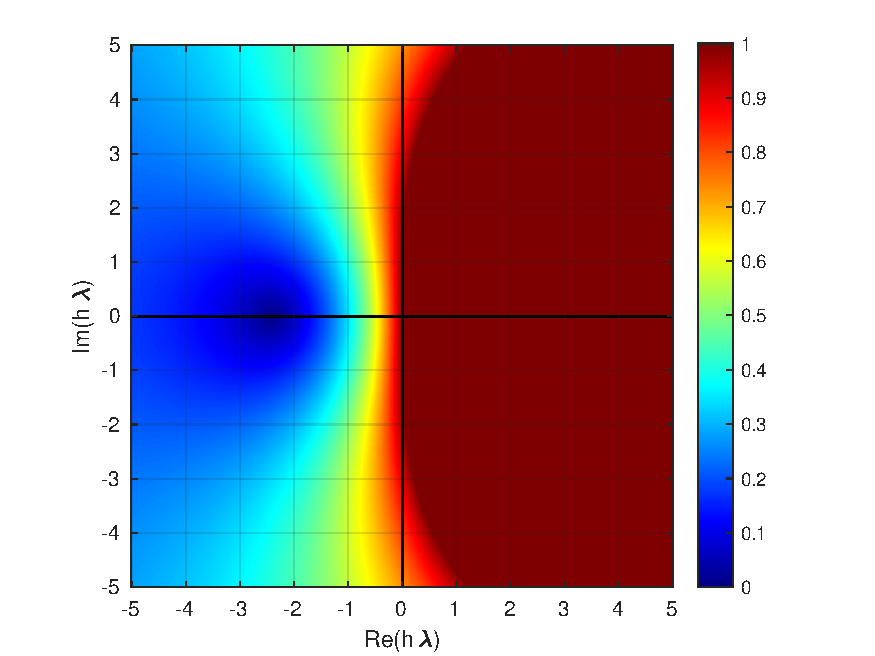
\includegraphics[width=0.7\linewidth]{images/8/8_2_stability_regions.pdf} 
    \caption{Values of $R(h\lambda)$ for the Explicit Singly-Diagonally Implicit Runge-Kutta 23 method}
    \label{8_2_stability_regions}
\end{figure}


\subsection{Implement ESDIRK23 with variable step size.}
For this part, we'll use the ESDIRK library given in the course codes. This library lets you select from different ESDIRK methods and implements them with adaptive step size. THe implementation is shown below:

\begin{lstlisting}[caption = ESDIRK23 method with adaptive time step size, captionpos=b, label=8_ESDIRK23_adaptive]
function [Tout,Xout,Gout,info,stats] = ESDIRK(fun,jac,t0,tf,x0,h0,absTol,relTol,Method,varargin)

%% ESDIRK23 Parameters 
%=========================================================================
% Runge-Kutta method parameters
switch Method
    case 'ESDIRK12'
        gamma = 1;
        AT = [0 0;0 gamma];
        c  = [0; 1];
        b  = AT(:,2);
        bhat = [1/2; 1/2];
        d  = b-bhat;
        p  = 1;
        phat = 2;
        s = 2;
    case 'ESDIRK23'
        gamma = 1-1/sqrt(2);
        a31 = (1-gamma)/2;
        AT = [0 gamma a31;0 gamma a31;0 0 gamma];
        c  = [0; 2*gamma; 1];
        b  = AT(:,3);
        bhat = [    (6*gamma-1)/(12*gamma); ...
            1/(12*gamma*(1-2*gamma)); ...
            (1-3*gamma)/(3*(1-2*gamma))    ];
        d  = b-bhat;
        p  = 2;
        phat = 3;
        s = 3;
    case 'ESDIRK34'
        gamma = 0.43586652150845899942;
        a31 = 0.14073777472470619619;
        a32 = -0.1083655513813208000;
        AT  = [0 gamma a31   0.10239940061991099768;
            0 gamma a32   -0.3768784522555561061;
            0 0     gamma 0.83861253012718610911;
            0 0     0     gamma                 ];
        c  = [0; 0.87173304301691799883; 0.46823874485184439565; 1];
        b  = AT(:,4);
        bhat = [0.15702489786032493710;
            0.11733044137043884870;
            0.61667803039212146434;
            0.10896663037711474985];
        d = b-bhat;
        p = 3;
        phat = 4;
        s = 4;
end


% error and convergence controller
epsilon = 0.8;
tau = 0.1*epsilon; %0.005*epsilon;
itermax = 20;
ke0 = 1.0/phat;
ke1 = 1.0/phat;
ke2 = 1.0/phat;
alpharef = 0.3;
alphaJac = -0.2;
alphaLU  = -0.2;
hrmin = 0.01;
hrmax = 10;
%========================================================================
tspan = [t0 tf]; % carsten
info = struct(...
            'Method',    Method,  ... % carsten
            'nStage',    s,       ... % carsten
            'absTol',    'dummy',  ... % carsten
            'relTol',    'dummy',  ... % carsten
            'iterMax',   itermax, ... % carsten
            'tspan',     tspan,   ... % carsten
            'nFun',      0, ...
            'nJac',      0, ...
            'nLU',       0, ...
            'nBack',     0, ...
            'nStep',     0, ...
            'nAccept',   0, ...
            'nFail',     0, ...
            'nDiverge',  0, ...
            'nSlowConv', 0);


        
%% Main ESDIRK Integrator
%========================================================================
nx = size(x0,1);
F = zeros(nx,s);
t = t0;
x = x0;
h = h0;

[F(:,1),g]  = feval(fun,t,x,varargin{:});
info.nFun = info.nFun+1;
[dfdx,dgdx] = feval(jac,t,x,varargin{:});
info.nJac = info.nJac+1;
FreshJacobian = true;
if (t+h)>tf
    h = tf-t;
end
hgamma = h*gamma;
dRdx = dgdx - hgamma*dfdx;
[L,U,pivot] = lu(dRdx,'vector');
info.nLU = info.nLU+1;
hLU = h;

FirstStep = true;
ConvergenceRestriction = false;
PreviousReject = false;
iter = zeros(1,s);

% Output
chunk = 100;
Tout = zeros(chunk,1);
Xout = zeros(chunk,nx);
Gout = zeros(chunk,nx); 

Tout(1,1) = t;
Xout(1,:) = x.';
Gout(1,:) = g.';

while t<tf
    info.nStep = info.nStep+1;
    %=====================================================================
    % A step in the ESDIRK method
    i=1;   
    diverging = false;
    SlowConvergence = false; % carsten
    alpha = 0.0;
    Converged = true;
    while (i<s) && Converged
        % Stage i=2,...,s of the ESDIRK Method
        i=i+1;
        phi = g + F(:,1:i-1)*(h*AT(1:i-1,i));

        % Initial guess for the state
         if i==2
             dt = c(i)*h;
             G = g + dt*F(:,1);
             X = x + dgdx\(G-g);
         else
             dt = c(i)*h;
             G  = g + dt*F(:,1);
             X  = x + dgdx\(G-g);
         end
        T = t+dt;
            
        [F(:,i),G] = feval(fun,T,X,varargin{:});
        info.nFun = info.nFun+1;
        R = G - hgamma*F(:,i) - phi;
%        rNewton = norm(R./(absTol + abs(G).*relTol),2)/sqrt(nx);
        rNewton = norm(R./(absTol + abs(G).*relTol),inf);
        Converged = (rNewton < tau);
        %iter(i) = 0; % original, if uncomment then comment line 154: iter(:) = 0;
        % Newton Iterations
        while ~Converged && ~diverging && ~SlowConvergence%iter(i)<itermax
            iter(i) = iter(i)+1;
            dX = U\(L\(R(pivot,1)));
            info.nBack = info.nBack+1;
            X = X - dX;
            rNewtonOld = rNewton;
            [F(:,i),G] = feval(fun,T,X,varargin{:});
            info.nFun = info.nFun+1;
            R = G - hgamma*F(:,i) - phi;
%            rNewton = norm(R./(absTol + abs(G).*relTol),2)/sqrt(nx);
            rNewton = norm(R./(absTol + abs(G).*relTol),inf);
            alpha = max(alpha,rNewton/rNewtonOld);
            Converged = (rNewton < tau);
            diverging = (alpha >= 1);
            SlowConvergence = (iter(i) >= itermax); % carsten
            %SlowConvergence = (alpha >= 0.5); % carsten
            %if (iter(i) >= itermax), i, iter(i), Converged, diverging, pause, end % carsten
        end
        %diverging = (alpha >= 1); % original, if uncomment then comment line 142: diverging = (alpha >= 1)*i;
        diverging = (alpha >= 1)*i; % carsten, recording which stage is diverging
    end
    %if diverging, i, iter, pause, end
    nstep = info.nStep;
    stats.t(nstep) = t;
    stats.h(nstep) = h;
    stats.r(nstep) = NaN;
    stats.iter(nstep,:) = iter;
    stats.Converged(nstep) = Converged;
    stats.Diverged(nstep)  = diverging;
    stats.AcceptStep(nstep) = false;
    stats.SlowConv(nstep)  = SlowConvergence*i; % carsten, recording which stage is converging to slow (reaching maximum no. of iterations)
    iter(:) = 0; % carsten
    %=====================================================================
    % Error and Convergence Controller
    if Converged
        % Error estimation
        e = F*(h*d);
%        r = norm(e./(absTol + abs(G).*relTol),2)/sqrt(nx);
        r = norm(e./(absTol + abs(G).*relTol),inf);
        CurrentStepAccept = (r<=1.0);
        r = max(r,eps);
        stats.r(nstep) = r;
        % Step Length Controller
        if CurrentStepAccept
            stats.AcceptStep(nstep) = true;
            info.nAccept = info.nAccept+1;
            if FirstStep || PreviousReject || ConvergenceRestriction
                % Aymptotic step length controller
                hr = 0.75*(epsilon/r)^ke0; 
            else
                % Predictive controller
                s0 = (h/hacc);
                s1 = max(hrmin,min(hrmax,(racc/r)^ke1));
                s2 = max(hrmin,min(hrmax,(epsilon/r)^ke2));
                hr = 0.95*s0*s1*s2;
            end
            racc = r;
            hacc = h;
            FirstStep = false;
            PreviousReject = false;
            ConvergenceRestriction = false;
            
            % Next Step
            t = T;
            x = X;
            g = G;
            F(:,1) = F(:,s);            
            
        else % Reject current step
            info.nFail = info.nFail+1;
            if PreviousReject
                kest = log(r/rrej)/(log(h/hrej));
                kest = min(max(0.1,kest),phat);
                hr   = max(hrmin,min(hrmax,((epsilon/r)^(1/kest))));
            else
                hr = max(hrmin,min(hrmax,((epsilon/r)^ke0)));
            end
            rrej = r;
            hrej = h;
            PreviousReject = true;
        end
   
        % Convergence control
        halpha = (alpharef/alpha);
        if (alpha > alpharef)
            ConvergenceRestriction = true;
            if hr < halpha
                h = max(hrmin,min(hrmax,hr))*h;
            else
                h = max(hrmin,min(hrmax,halpha))*h;
            end
        else
            h = max(hrmin,min(hrmax,hr))*h;
        end
        h = max(1e-8,h);
        if (t+h) > tf
            h = tf-t;
        end
        
        % Jacobian Update Strategy
        FreshJacobian = false;
        if alpha > alphaJac
            [dfdx,dgdx] = feval(jac,t,x,varargin{:});
            info.nJac = info.nJac+1;
            FreshJacobian = true;
            hgamma = h*gamma;
            dRdx = dgdx - hgamma*dfdx; 
            [L,U,pivot] = lu(dRdx,'vector');
            info.nLU = info.nLU+1;
            hLU = h;
        elseif (abs(h-hLU)/hLU) > alphaLU 
            hgamma = h*gamma;
            dRdx = dgdx-hgamma*dfdx;
            [L,U,pivot] = lu(dRdx,'vector');
            info.nLU = info.nLU+1;
            hLU = h;
        end        
    else % not converged
        info.nFail=info.nFail+1;
        CurrentStepAccept = false;
        ConvergenceRestriction = true;
        if FreshJacobian && diverging
            h = max(0.5*hrmin,alpharef/alpha)*h;
            info.nDiverge = info.nDiverge+1;
        elseif FreshJacobian
            if alpha > alpharef
                h = max(0.5*hrmin,alpharef/alpha)*h;
            else
                h = 0.5*h;
            end
        end
        if ~FreshJacobian
            [dfdx,dgdx] = feval(jac,t,x,varargin{:});
            info.nJac = info.nJac+1;
            FreshJacobian = true;
        end
        hgamma = h*gamma;
        dRdx = dgdx - hgamma*dfdx;
        [L,U,pivot] = lu(dRdx,'vector');
        info.nLU = info.nLU+1;
        hLU = h;
    end
    
    %=====================================================================
    % Storage of variables for output
    
    if CurrentStepAccept
       nAccept = info.nAccept;
       if nAccept > length(Tout);
           Tout = [Tout; zeros(chunk,1)];
           Xout = [Xout; zeros(chunk,nx)];
           Gout = [Gout; zeros(chunk,nx)];
       end
       Tout(nAccept,1) = t;
       Xout(nAccept,:) = x.';
       Gout(nAccept,:) = g.';
    end
end
info.nSlowConv = length(find(stats.SlowConv)); % carsten
nAccept = info.nAccept;
Tout = Tout(1:nAccept,1);
Xout = Xout(1:nAccept,:);
Gout = Gout(1:nAccept,:);

end

\end{lstlisting}

%%%%%%%%%%%%%%%%%%%%%%%%%%%%%%%%%%%%%%%%%%%%%%%%%%%%%%%%%%%%%%%%%%%%%%%%%%%%%%%%%%%%%%%%%%%%%%%%%%%
\subsection{Test your algorithms on the Van der Pol problem \texorpdfstring{($\mathbf{\mu = 1.5}$ and $\mathbf{\mu = 15}$, $\mathbf{x_0 = [1.0;1.0]}$).}{(mu = 1.5 and mu = 15, x0 = [1.0;1.0]).}}
The results for the Van der Pol problem using ESDIRK 23 method are shown below. We can see that the convergence of the solution is pretty good, but what's more interesting is the improvement in the "stiff" version of the problem ($\mu = 15$). Here, the method uses even less function evaluations than in the non-stiff problem, achieving also a great convergence. The only drawback of the method is working with non-stiff problems. Comparing Table \ref{8_4_adaptive_mu_1_5_table} with the results for Dormand-Prince 5(4) (Table \ref{7_4_adaptive_mu_1_5_table}), we can see how the number of evaluations increases considerably. For this type of problems, we can achieve better accuracy using an explicit method.

It's worth mentioning that the values of $r$ shown go past 1 because the algorithm used (\ref{8_ESDIRK23_adaptive}) stores every value of $h$ and $r$, not only the ones accepted. 
\begin{figure}[H]
    \centering
    \makebox[\textwidth][c]{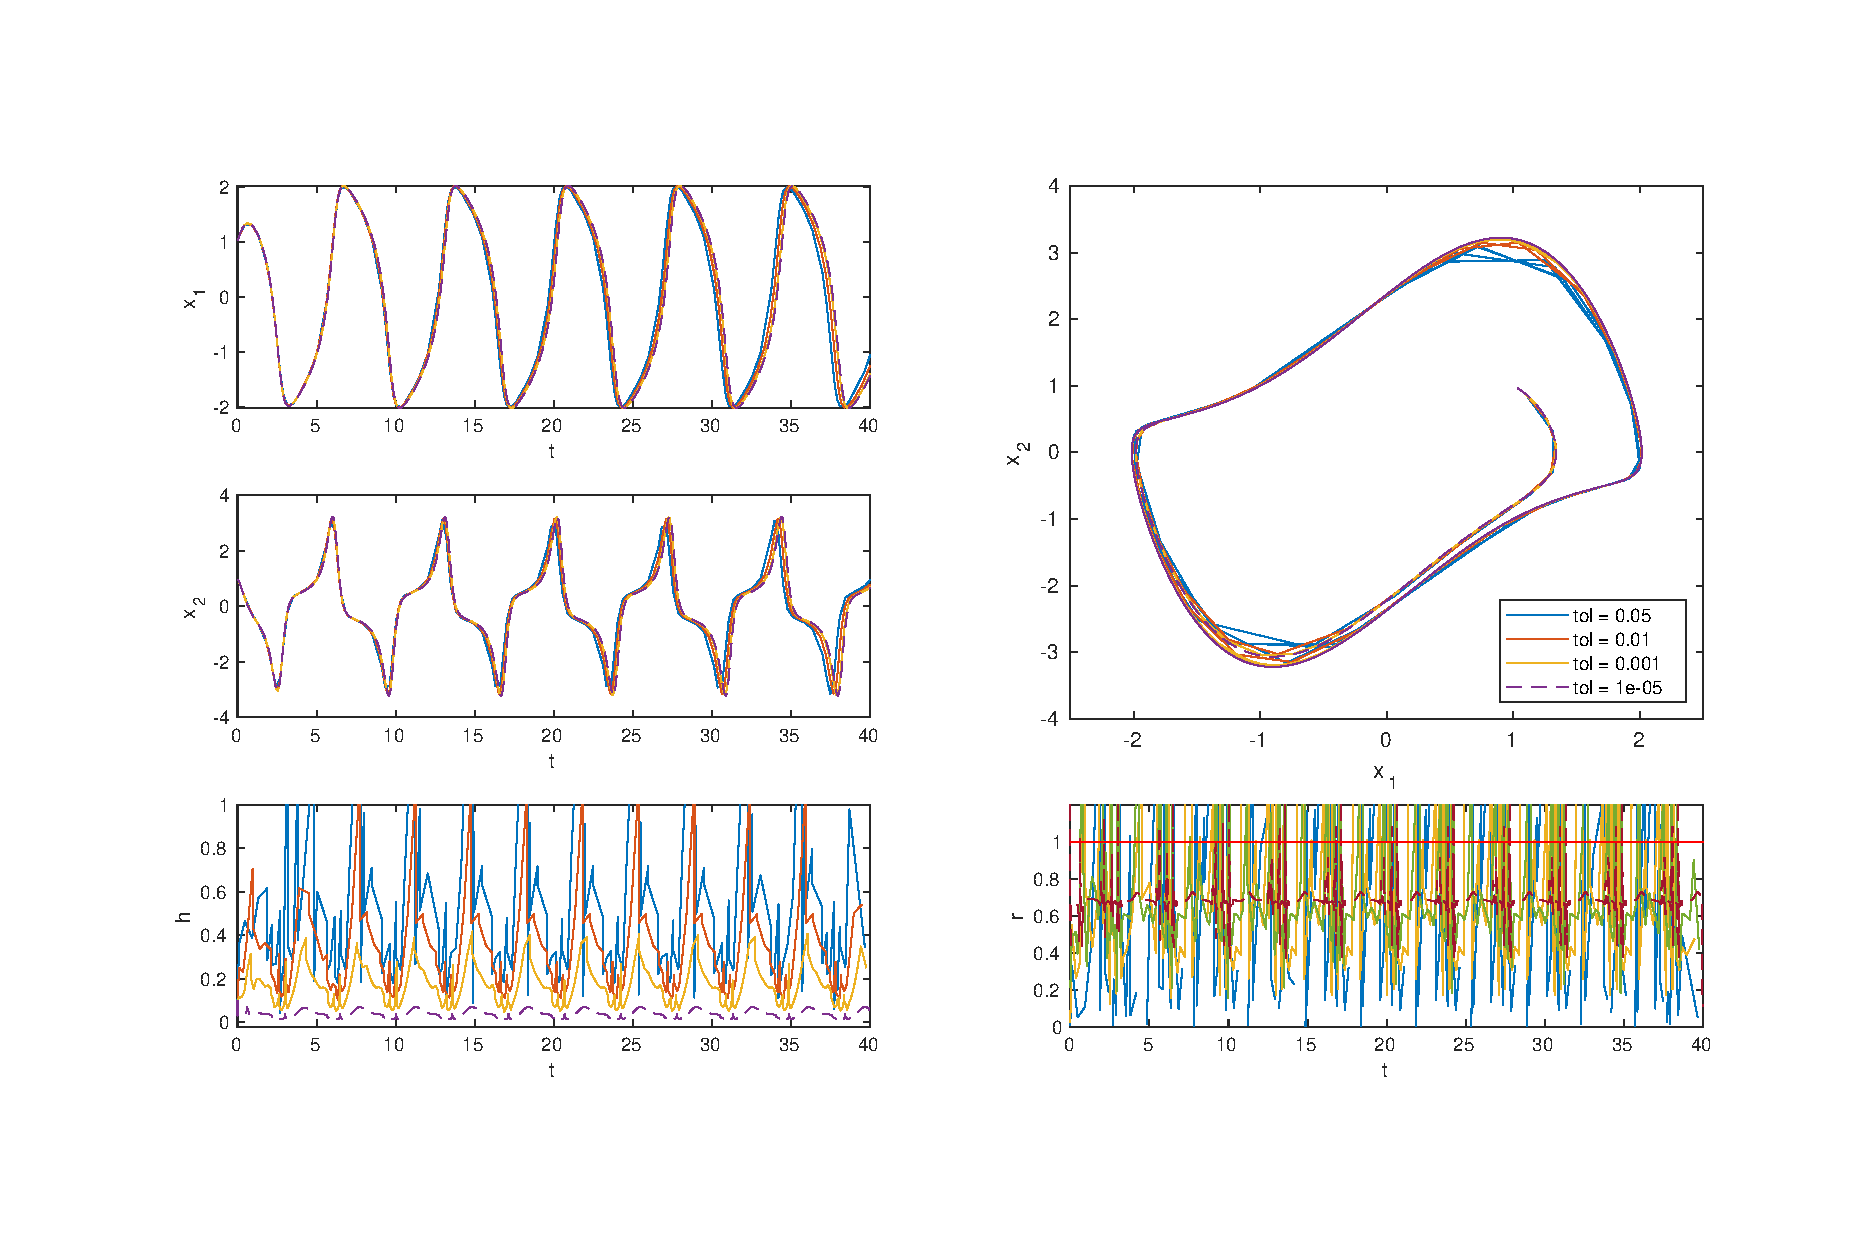
\includegraphics[width=1.25\textwidth]{images/8/8_4_adaptive_mu_1_5.pdf}}
    \caption{Solution for the Van der Pol problem ($\mathit{\mu = 1.5}$) using ESDIRK23 with adaptive step size}
    \label{8_4_mu_1_5}
\end{figure}

\begin{table}[H]
    \centering
    \begin{tabular}{@{}l|cccc@{}}
    \toprule
    Tolerances           & 0.05 & 0.01 & 0.001 & 1e-05 \\ \midrule
    Function evaluations & 1196 & 1417 & 1864  & 6197  \\
    Calculated steps     & 178  & 220  & 356   & 1397  \\
    Accepted steps       & 117  & 158  & 312   & 1372  \\
    Rejected steps       & 61   & 62   & 44    & 25    \\ \bottomrule
    \end{tabular}
    \caption{Parameters of the ESDIRK23 with adaptive step size for the Van der Pol problem ($\mathit{\mu = 1.5}$)}
    \label{8_4_adaptive_mu_1_5_table}
\end{table}

\begin{figure}[H]
    \centering
    \makebox[\textwidth][c]{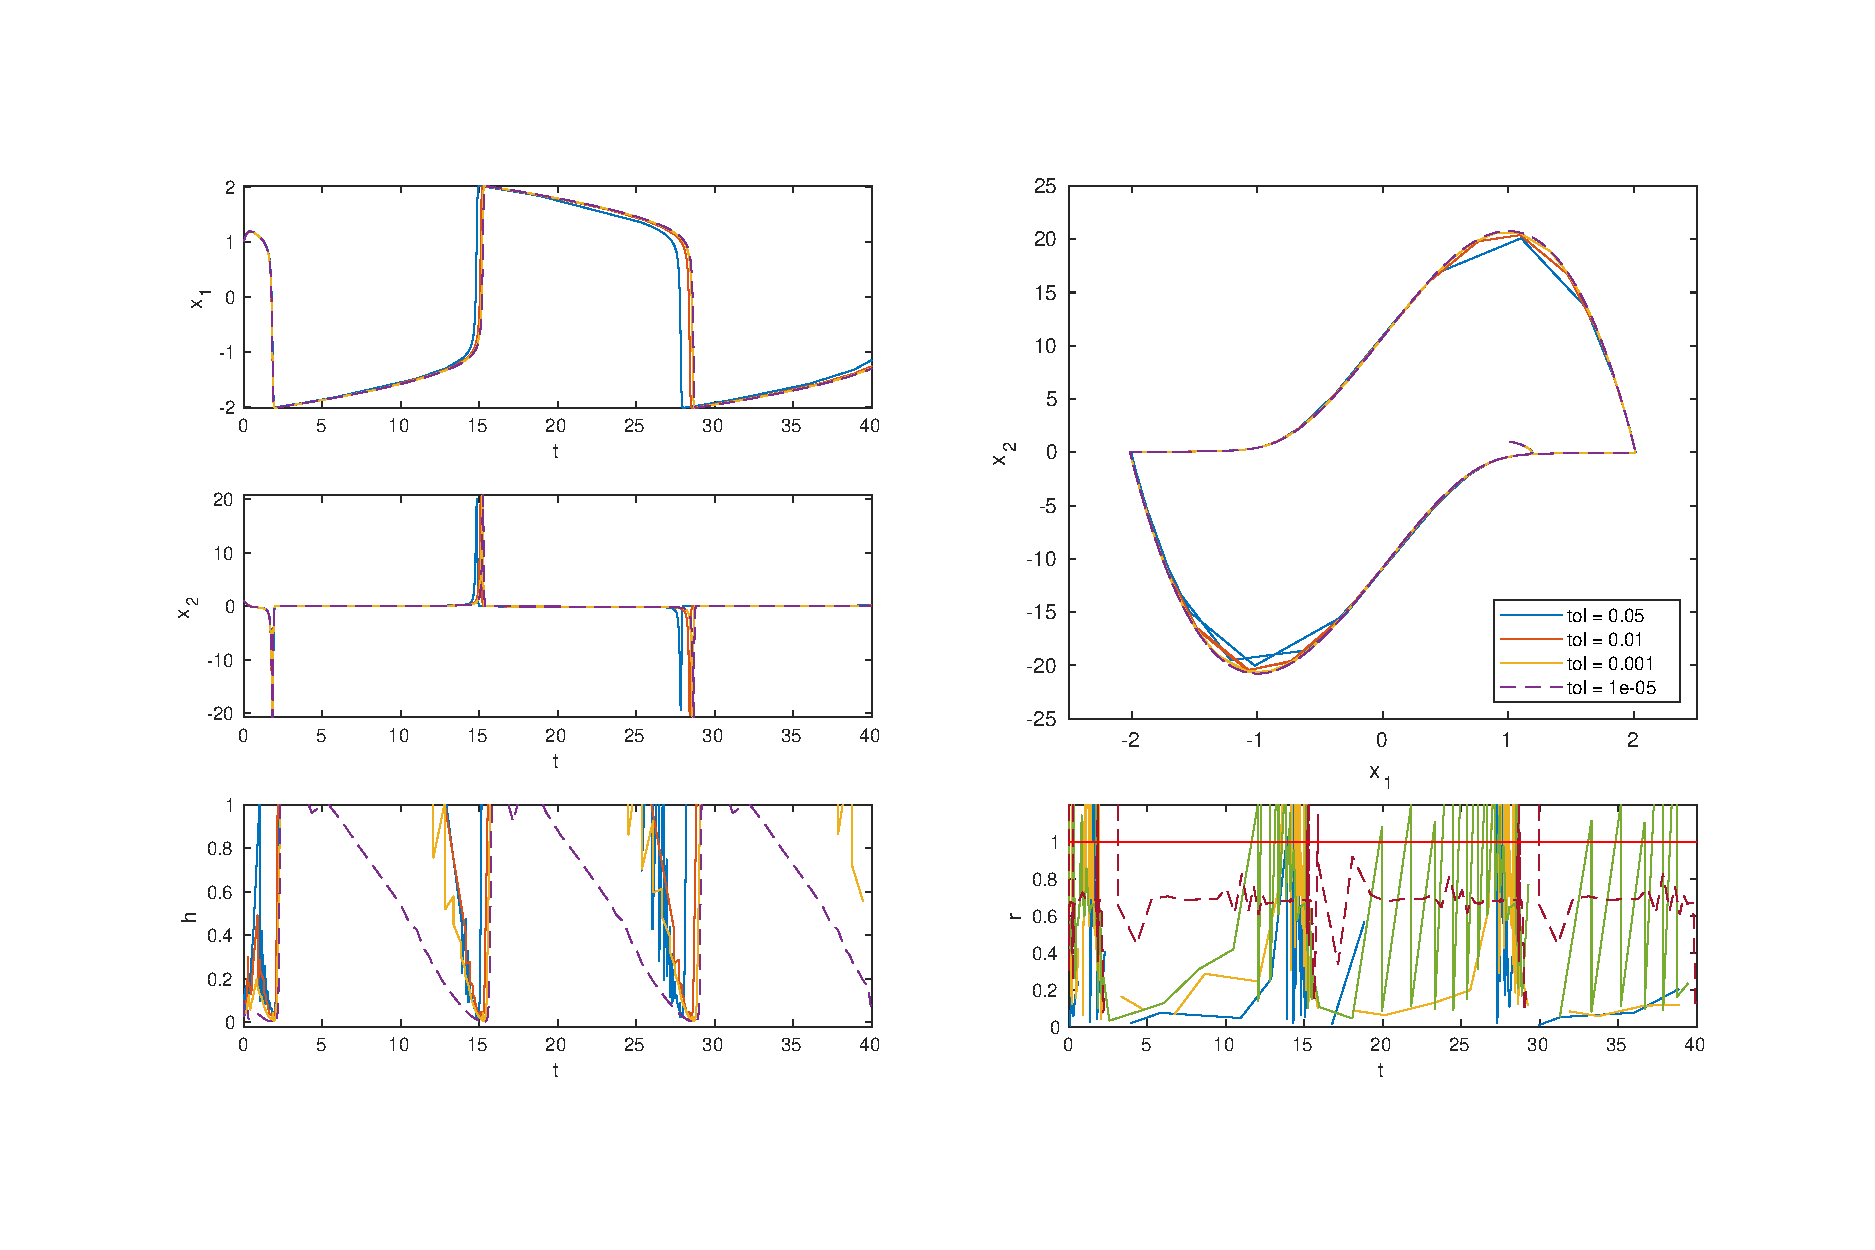
\includegraphics[width=1.25\textwidth]{images/8/8_4_adaptive_mu_15.pdf}}
    \caption{Solution for the Van der Pol problem ($\mathit{\mu = 15}$) using ESDIRK23 with adaptive step size}
    \label{8_4_mu_15}
\end{figure}

\begin{table}[H]
    \centering
    \begin{tabular}{@{}l|cccc@{}}
    \toprule
    Tolerances           & 0.05 & 0.01 & 0.001 & 1e-05 \\ \midrule
    Function evaluations & 740  & 814  & 1325  & 3763  \\
    Calculated steps     & 115  & 127  & 223   & 802   \\
    Accepted steps       & 78   & 98   & 188   & 782   \\
    Rejected steps       & 37   & 29   & 35    & 20    \\ \bottomrule
    \end{tabular}
    \caption{Parameters of the ESDIRK23 with adaptive step size for the Van der Pol problem ($\mathit{\mu = 15}$)}
    \label{8_4_adaptive_mu_15_table}
\end{table}


%%%%%%%%%%%%%%%%%%%%%%%%%%%%%%%%%%%%%%%%%%%%%%%%%%%%%%%%%%%%%%%%%%%%%%%%%%%%%%%%%%%%%%%%%%%%%%%%%%%
\subsection{Test  your  algorithms  on  the  adiabatic  CSTR  problem  described  in  the papers uploaded to Learn (3D-version and 1D-version).}
Not surprisingly, the ESDIRK 23 also shows great performance on the CSTR problem. It captures the solution greatly, and handles the stiffness when $F$ is low amazingly.

\begin{figure}[H]
    \centering
    \makebox[\textwidth][c]{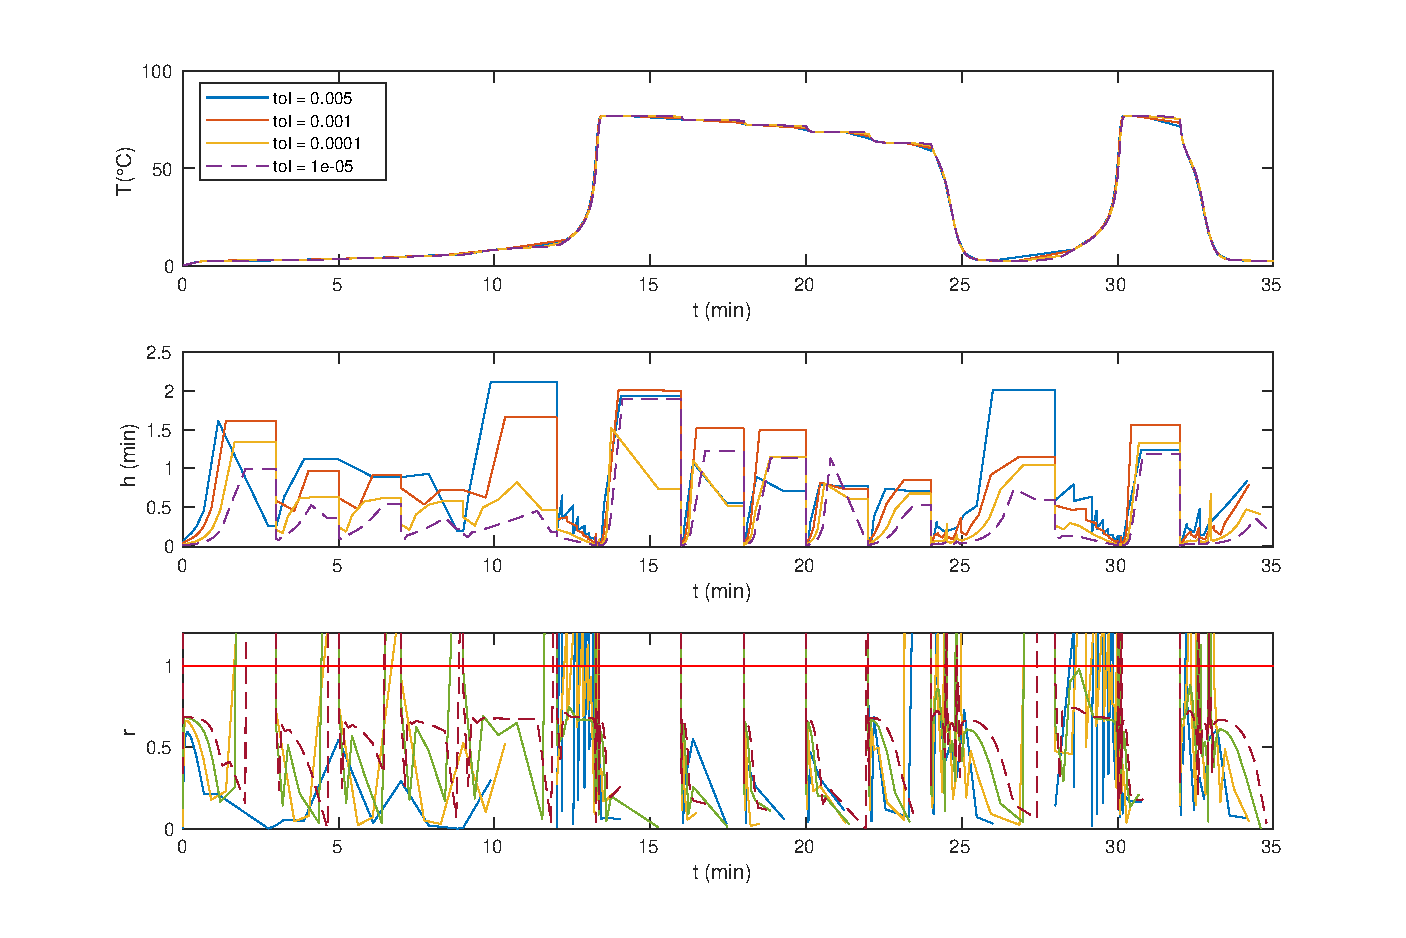
\includegraphics[width=1\textwidth]{images/8/8_5_3D_tols.pdf}}
    \caption{Solution for the CSTR 3D problem using ESDRIK 23 with adaptive step size}
    \label{8_5_3D_tols}
\end{figure}

\begin{table}[H]
    \centering
    \begin{tabular}{@{}l|cccc@{}}
    \toprule
    Tolerances           & 0.005 & 0.001 & 0.0001 & 1e-05 \\ \midrule
    Function evaluations & 878   & 1095  & 1497   & 2454  \\
    Calculated steps     & 129   & 171   & 267    & 495   \\
    Accepted steps       & 90    & 120   & 227    & 455   \\
    Rejected steps       & 39    & 51    & 40     & 40    \\ \bottomrule
    \end{tabular}
    \caption{Parameters of the ESDIRK 23 with adaptive step size for the CSTR 3D problem}
    \label{8_5_3D_tols_table}
\end{table}

\begin{figure}[H]
    \centering
    \makebox[\textwidth][c]{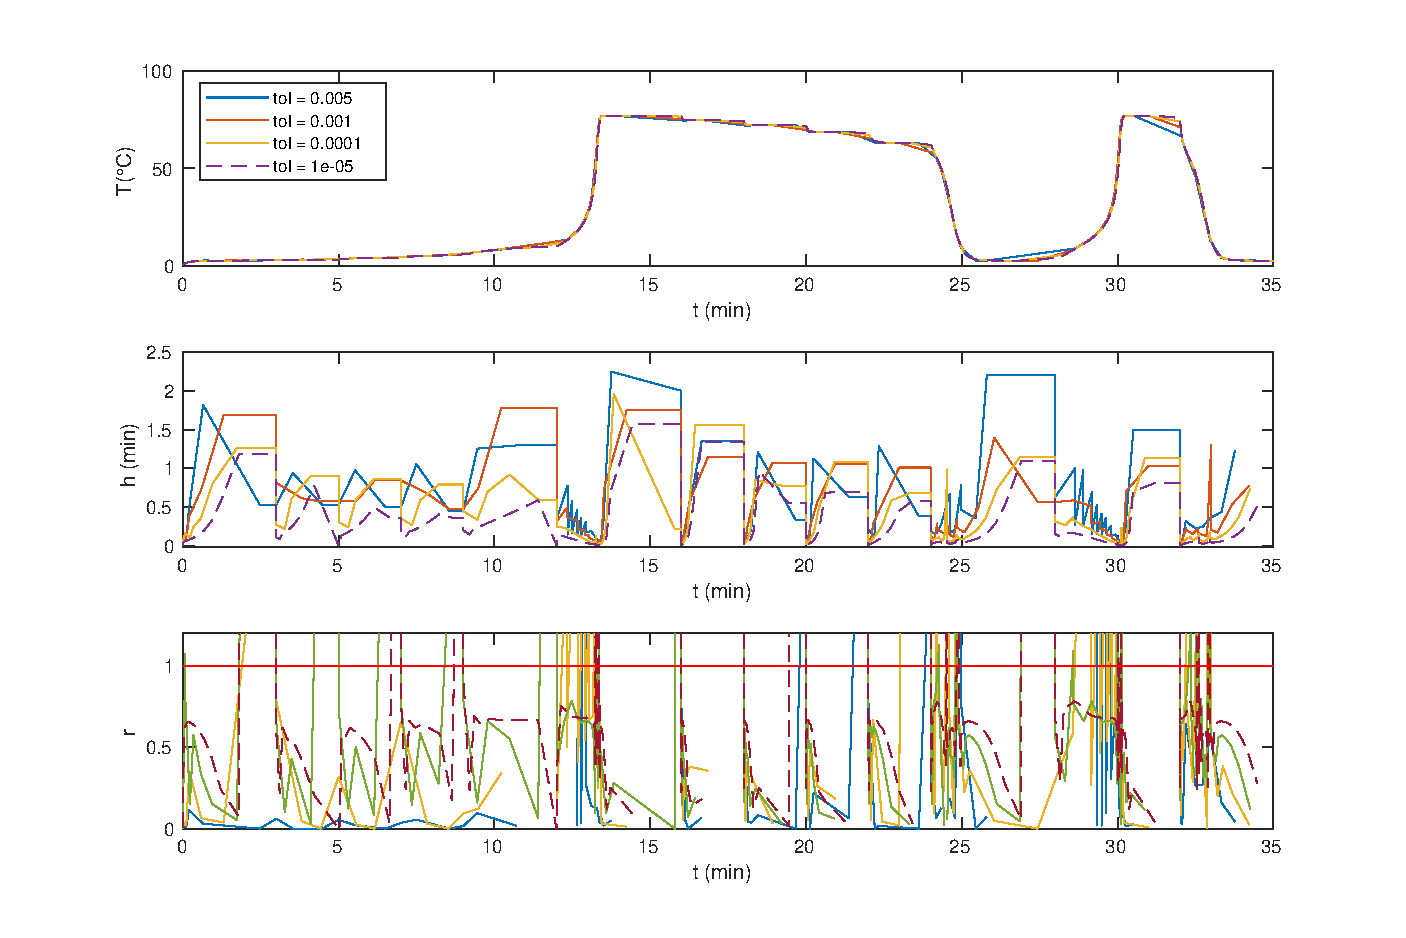
\includegraphics[width=1\textwidth]{images/8/8_5_1D_tols.pdf}}
    \caption{Solution for the CSTR 1D problem using ESDIRK 23 with adaptive step size}
    \label{8_5_1D_tols}
\end{figure}

\begin{table}[H]
    \centering
    \begin{tabular}{@{}l|cccc@{}}
    \toprule
    Tolerances           & 0.005 & 0.001 & 0.0001 & 1e-05 \\ \midrule
    Function evaluations & 741   & 888   & 1226   & 1802  \\
    Calculated steps     & 107   & 130   & 201    & 339   \\
    Accepted steps       & 78    & 91    & 157    & 305   \\
    Rejected steps       & 29    & 39    & 44     & 34    \\ \bottomrule
    \end{tabular}
    \caption{Parameters of the ESDIRK 23 with adaptive step size for the CSTR 1D problem}
    \label{8_5_1D_tols_table}
\end{table}


%%%%%%%%%%%%%%%%%%%%%%%%%%%%%%%%%%%%%%%%%%%%%%%%%%%%%%%%%%%%%%%%%%%%%%%%%%%%%%%%%%%%%%%%%%%%%%%%%%%
\subsection{Compare the solution and the number of function evaluations with your own explicit Runge-Kutta method to the other solvers that you have used in this exam problem.  Discuss when it is appropriate to use ESDIRK23 and illustrate that with an example you choose.}

For the sake of comparison, we will compare the ESDIRK23 with the same Matlab solvers we already used for the entirety of the project. We're interested in seeing if the ESDIRK23 could be a good alternative to the \code{ode15s} for the stiff cases while still being usable for non-stiff problems (compared to \code{ode45}).

The results are very promising. The ESDIRK23 manages to achieve a convergent solution in the non-stiff problem (Figure \ref{8_6_mu_1_5}) without a huge increase in the number of function evaluations, specially if we take into account the huge difference between calculated steps. In the stiff Van der Pol problem it still has some more function evaluations than the \code{ode15s}, but nothing considering the difference all the other explicit methods had.

It's also curious to see how in the CSTR problem the method performs a lot less steps than the other ODEs, achieving overall good performance and failing a bit on the steps. This behaviour is easily solved by cranking a little bit tighter the tolerance. Overall, we can conclude that the ESDIRK23 achieves a good balance between accuracy and computation for both stiff and non-stiff problems.

\begin{figure}[H]
    \centering
    \makebox[\textwidth][c]{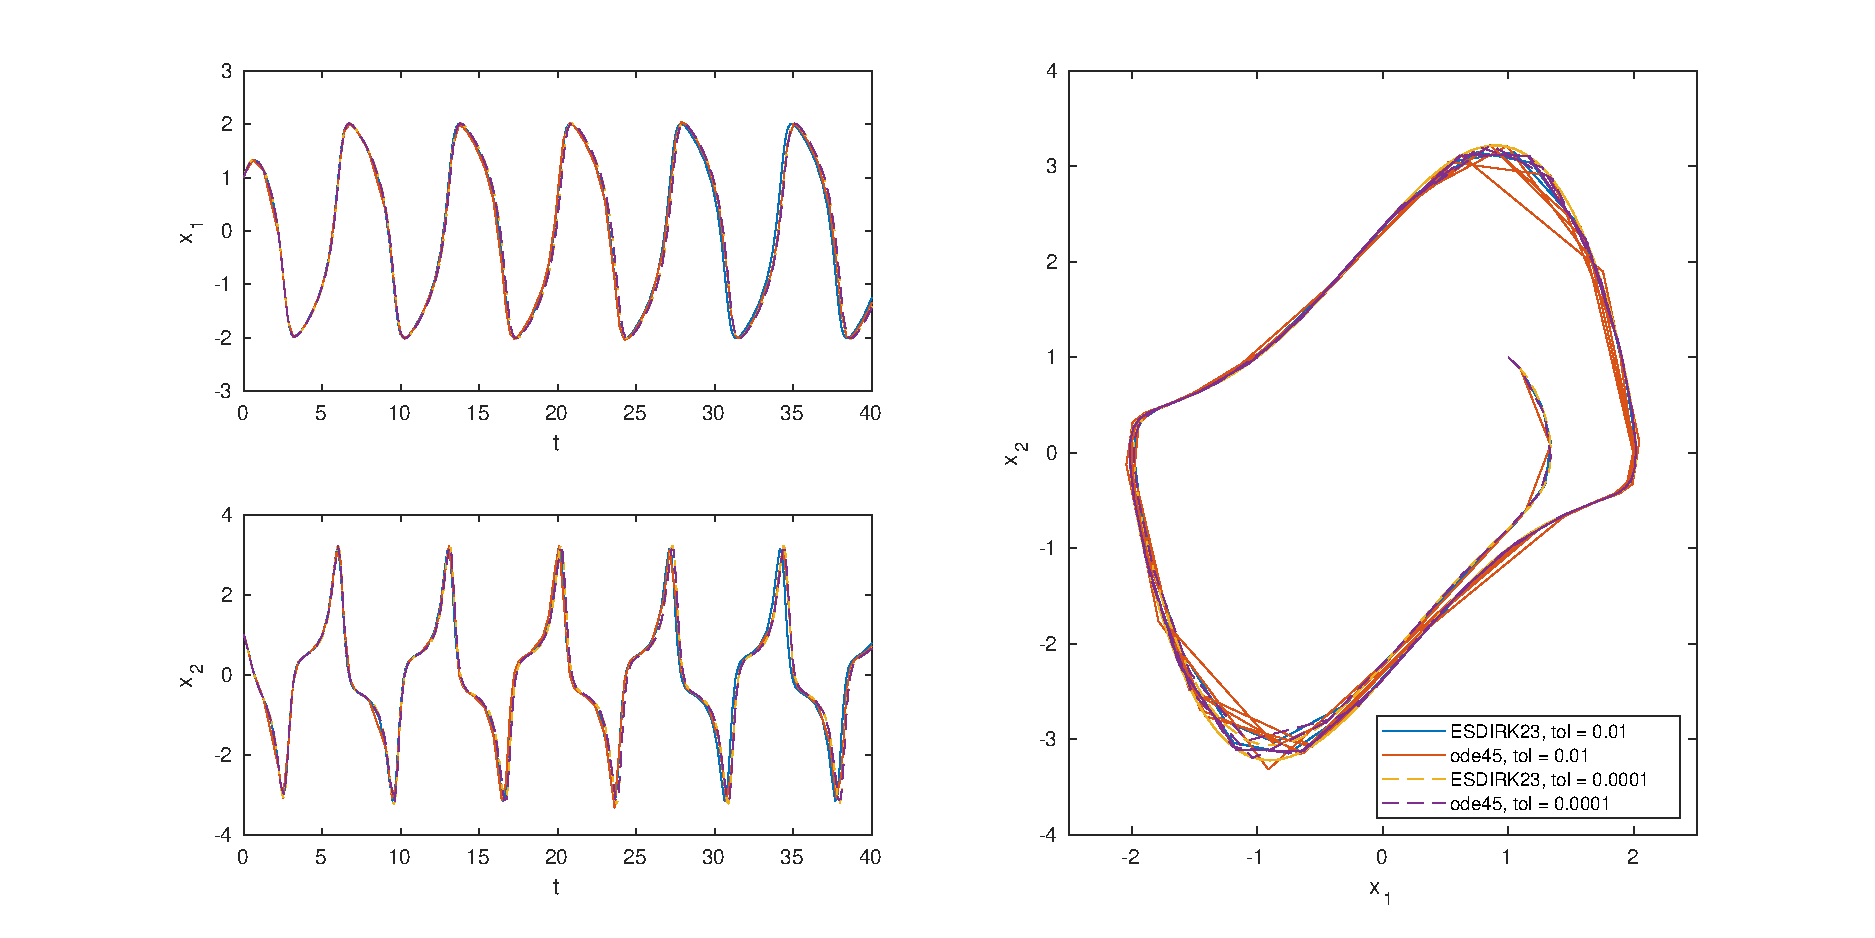
\includegraphics[width=1.25\textwidth]{images/8/8_6_mu_1_5.pdf}}
    \caption{Solution for the Van der Pol problem ($\mathit{\mu = 1.5}$) using ESDIRK23 vs. \code{ode45}}
    \label{8_6_mu_1_5}
\end{figure}

\begin{table}[H]
    \centering
    \begin{tabular}{@{}l|cc|cc@{}}
    \toprule
    \textbf{Method}      & \multicolumn{2}{c|}{\textbf{ESDIRK23}} & \multicolumn{2}{c}{\textbf{ode45}} \\
    Tolerances           & 0.01              & 0.0001             & 0.01            & 0.0001           \\ \midrule
    Function evaluations & 1417              & 3250               & 787             & 1357             \\
    Calculated steps     & 220               & 679                & 131             & 226              \\
    Accepted steps       & 158               & 645                & 100             & 180              \\
    Rejected steps       & 62                & 34                 & 31              & 46               \\ \bottomrule
    \end{tabular}
    \caption{Parameters of the ESDIRK23 vs. \code{ode45} for the Van der Pol problem ($\mathit{\mu = 1.5}$)}
    \label{8_6_adaptive_mu_1_5_table}
\end{table}

\begin{figure}[H]
    \centering
    \makebox[\textwidth][c]{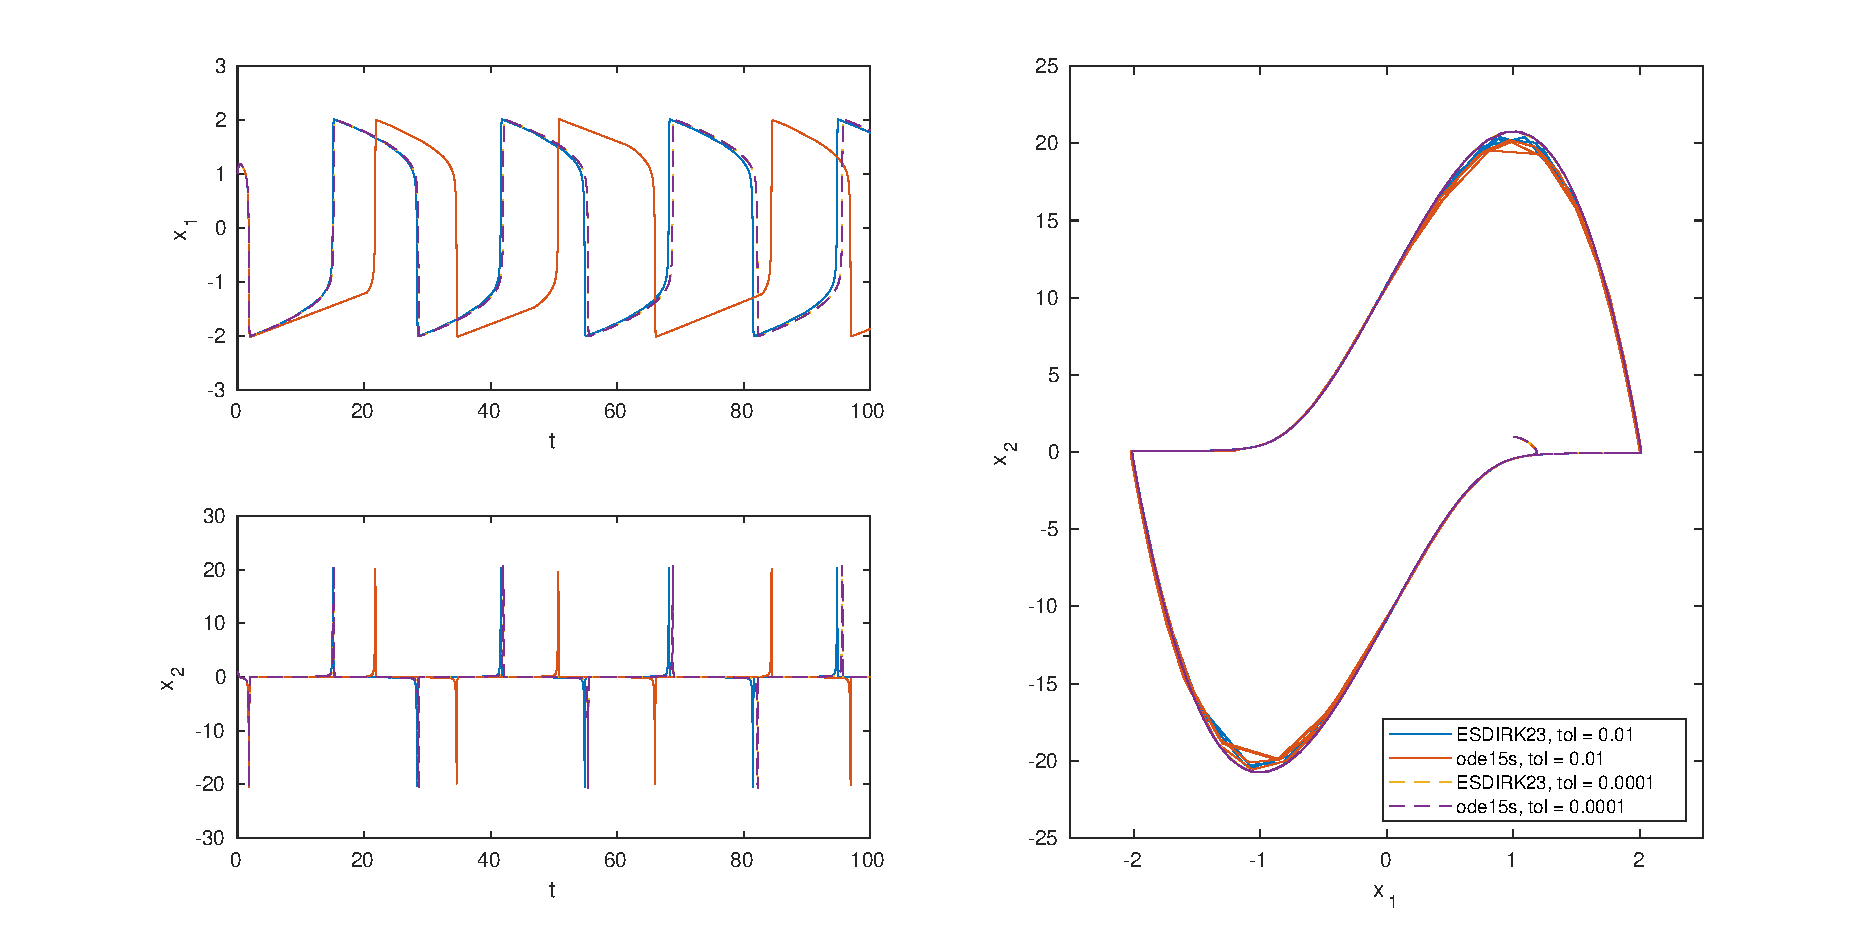
\includegraphics[width=1.25\textwidth]{images/8/8_6_mu_15.pdf}}
    \caption{Solution for the Van der Pol problem ($\mathit{\mu = 15}$) using ESDIRK23 vs. \code{ode15s}}
    \label{8_6_mu_15}
\end{figure}

\begin{table}[H]
    \centering
    \begin{tabular}{@{}l|cc|cc@{}}
    \toprule
    \textbf{Method}      & \multicolumn{2}{c|}{\textbf{ESDIRK23}} & \multicolumn{2}{c}{\textbf{ode15s}} \\
    Tolerances           & 0.01              & 0.0001             & 0.01            & 0.0001           \\ \midrule
    Function evaluations & 2112              & 5111               & 1273            & 2780             \\
    Calculated steps     & 327               & 990                & 558             & 1327             \\
    Accepted steps       & 250               & 947                & 411             & 1094             \\
    Rejected steps       & 77                & 43                 & 147             & 233              \\ \bottomrule
    \end{tabular}
    \caption{Parameters of the ESDIRK23 vs. \code{ode15s} for the Van der Pol problem ($\mathit{\mu = 15}$)}
    \label{8_6_adaptive_mu_15_table}
\end{table}

\begin{figure}[H]
    \centering
    \begin{subfigure}{0.8\linewidth}
        \centering
        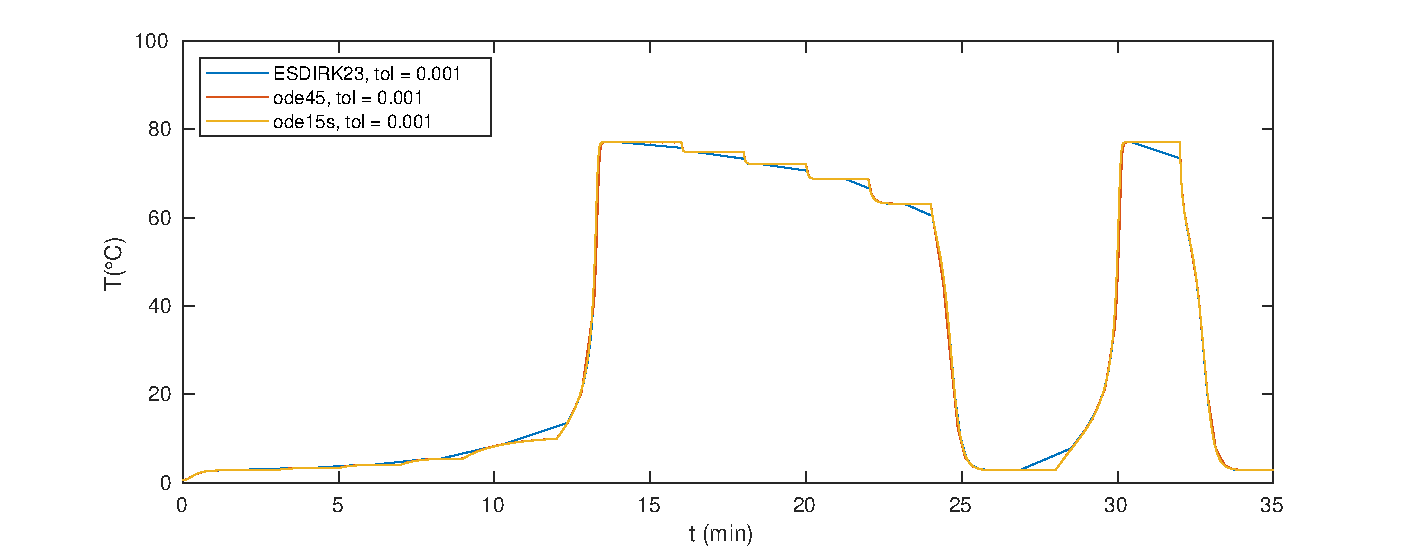
\includegraphics[width=1\linewidth]{images/8/8_6_3D.pdf} 
        \caption{CSTR 3D problem}
    \end{subfigure} \\
    \begin{subfigure}{0.8\linewidth}
        \centering
        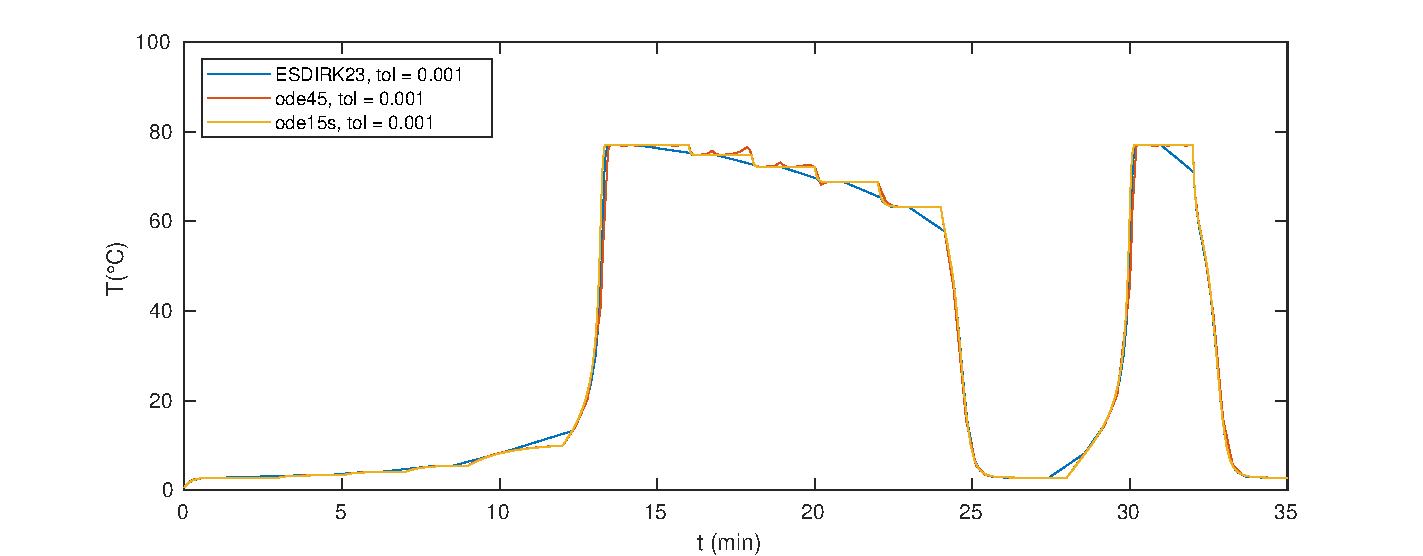
\includegraphics[width=1\linewidth]{images/8/8_6_1D.pdf}
        \caption{CSTR 1D problem}
    \end{subfigure}
    \caption{Solution for the CSTR problem using ESDIRK23 vs. \code{ode45} and \code{ode15s}}
    \label{8_6_3D_1D}
\end{figure}

\begin{table}[H]
    \centering
    \begin{tabular}{@{}l|c|c|c@{}}
    \toprule
    \textbf{Method}      & \textbf{ESDIRK23} & \textbf{ode45} & \textbf{ode15s} \\
    Tolerances           & 0.001             & 0.001          & 0.001           \\ \midrule
    Function evaluations & 1095              & 1447           & 770             \\
    Calculated steps     & 171               & 1520           & 2248            \\
    Accepted steps       & 120               & 210            & 340             \\
    Rejected steps       & 51                & 29             & 62              \\ \bottomrule
        \end{tabular}
        \caption{Parameters of the ESDIRK23 vs. \code{ode45} and \code{ode15s} for the CSTR-3D problem}
        \label{8_6_3D_table}
    \end{table}

\begin{table}[H]
    \centering
    \begin{tabular}{@{}l|c|c|c@{}}
    \toprule
    \textbf{Method}      & \multicolumn{1}{c|}{\textbf{ESDIRK23}} & \multicolumn{1}{c|}{\textbf{ode45}} & \multicolumn{1}{c}{\textbf{ode15s}} \\
    Tolerances           & 0.001                                  & 0.001                               & 0.001                               \\ \midrule
    Function evaluations & 888                                    & 1315                                & 538                                 \\
    Calculated steps     & 130                                    & 1395                                & 1604                                \\
    Accepted steps       & 91                                     & 195                                 & 241                                 \\
    Rejected steps       & 39                                     & 22                                  & 48                                  \\ \bottomrule
    \end{tabular}
    \caption{Parameters of the ESDIRK23 vs. \code{ode45} and \code{ode15s} for the CSTR-1D problem}
    \label{8_6_1D_table}
\end{table}

